\section{Exploration de uintr}
\label{sec:exploreUintr}

Pour cette partir j'ai utiliser des connaissance personnel autour du système, du développement noyau, de Linux... et aussi ce que j'ai appris en cours de \emph{programmation système}, de \emph{système d'exploitation} et \emph{architecture des ordinateurs}.

\subsection{Prérequis est accès}
\label{requirements}

Pour utilisé le mécanisme d'interruption en espace utilisateur il faut donc avoir accès à un CPU \intel{} Sapphire Rapids.
Comme ils sont sortie très récemment ils sont assez difficile d'accès.
Atos nous a, non sans difficulté donné accès, à une machine qui possède 2 CPU \intel{} Sapphire Rapids qui sont des \intel{} Xeon\textsuperscript{\tiny{\textregistered}} Platinum 8470.
Ils y a eu plusieurs difficulté pour avoir une machine, pour quelle sois installer et pour quelle sois dans un réseau au quelle on puisse accédé depuis l'Inria.
On à donc eu un accès VPN qui utilisé l'ancien système de VPN car le nouveau ne fonctionné pas.
Nous avons donc eu accès à la machine environ deux mois et demi après le début du stage.
La machine est déjà configuré avec le système d'exploitation Red Hat Enterprise Linux (RHEL) 9.1.
Elle possède deux carte BIX v2 que nous n'avons pas utilisé lors du stage.

Il faut aussi avoir une version patché du noyaux linux avec le support du nouveau mécanisme.
Cette version patché n'est pas encore disponible dans la branche principal du noyau.
Elle est disponible sur le GitHub d'\intel{}. Nous avons donc télécharger cette version patché.
Nous l'avons compiler et installer sur la machine.
Lors de la compilation il faut activé le support des uintr (Voir figure en annexes\ref{fig:enableFeaturesInConfigMenu}).
Il est aussi possible d'activé le support qu'un thread bloqué, c'est à dire pas ordonnancer ou dans une appel système interruptible, puisse recevoir une uintr.

Le mécanisme utilise de nouvelle instructions, il faut donc une version récente du compilateur GCC pour compiler les programme utilisateur qui utiliseront les uintr.
Il faut donc la version \textbf{11.3.0} ou plus récente de GCC, sur RHEL il faut la version \textbf{12.1.1} ou superieur.
Le support n'est pas encore disponible dans d'autre compilateur comme LLVM-Clang.
Pour compiler un programme utilisateur il faut précisé le flag de compilation \code{-muintr} pour les fichiers qui définisse un handler d'interruption ou qui utilise les nouvelles instructions.

\subsection{Fonctionnement des uintr}
\label{sec:uintr}

\subsubsection{Les interruptions}
\label{sec:interrupts}

Pour commencer nous allons voire comment les interruption matérielle fonctionnent.
Nous allons nous concentrer sur l'envois d'interruption entre deux processus qui sont fixer sur deux unité de calcul.
Pour fonctionné les CPU on une unité dédié au traitement des interruptions, l'APIC pour Advanced Programmable Interrupt Controller.
Cette APIC permet au système d'enregistré un handler pour chaque interruptions.
Pour ce faire le système définit un tableau \emph{IDT} (Interrupt Descriptor Table) qui contiens 256 entrées.
Donc 256 interruptions possible, les valeurs entre 0 et 255 sont aussi appelé vecteur.
Les vecteur compris entre 0 et 31 sont réservé pour les exceptions et interruption système, ce entre 32 et 127 sont réservé pour les interruptions pour les périphériques,
128 est réservé pour les appel système et entre 129 et 255 pour des utilisation varier.

Il est important de savoir que chaque unité de calcul (processeur logique) possède un \emph{APIC ID} physique.
Petit fun-fact le \emph{core ID} est un sous ensemble de l'\emph{APIC ID}.

Pour déclencher une interruption il y a quatre possibilités :

\begin{enumerate}
  \item Une exceptions déclencher par un processeur (e.g. division par zero, défaut de segmentation...).
  \item Une instruction comme \code{INT80 numSysCall} pour déclencher un appel système ou bien \code{INT3} pour définir un point d'arrêt, ou encore \code{INTO}, \code{BOUND} et \code{INT n}.
  \item Des pins du CPU dédier à la réception d'interruption lancer à partir d'un périphérique.
  \item Demander à l'APIC en lui même grâce à un registre ICR pour Interrupt Command Register.
  Il existe un ICR par vecteur il faut donc écrire l'\emph{APIC ID} du destinataire dans le ICR du vecteur que l'on veut déclencher.
  Seul le CPU et le noyau peuvent modifier les ICR.
\end{enumerate}

On vois bien que les IRQ fonctionne au niveau du noyau et du CPU.

Nous allons voir un exemple d'envoi d'IRQ entre 2 processus en cours d'exécution.
Tous d'abord l'initialisation ce fait au démarrage du système et consiste principalement à définir les handler noyau dans l'\emph{IDT}.
Au préalable il faut définir le vecteur utiliser, le handler noyau, la technique pour contacté le système et l'identification du récepteur (e.g. par un patch du noyau, par un module noyau...).

Nous allons maintenant voir les états de l'envois d'une IRQ montré sur la figure suivante \ref{fig:sendInt}.

\begin{enumerate}[label=\protect\circled{\arabic*}]
  \item Le récepteur fait un appel système pour indiquer au noyau comment il veut être avertie d'une interruption (e.g. un handler utilisateur, un descripteur de fichiers qu'il vas lire, un appel système bloquante, une zone mémoire où écrire...).
  \item l'émetteur peut donc avertir le noyau qu'il fau envoyer une interruption pour cela il peut utiliser un appel système ou écrire dans un descripteur de fichiers...
  \item Le noyau détermine l'unité de calcule ou ce trouve le récepteur. Pour cela il peut utiliser par exemple un \emph{PID} (Processus ID) donné par l'émetteur ou autre.
  Il vas donc pouvoir déterminer le \emph{APIC ID} de unité de calcul à interrompre.
  \item Le noyau écrit donc l'\emph{APIC ID} dans le \emph{ICR} d'un vecteur déterminer à l'avance. L'émetteur vas reprendre la main après un autre changement de contexte.
  \item L'APIC vas donc interrompre le récepteur qui vas donc stoppé sont exécution est passer dans le noyau.
  Une fois dans le noyau le handler vas ce déclencher et exécuté le code prévue au préalable (déclenchement d'un handler utilisateur, écrire dans un descripteur de fichiers, écrire dans une zone mémoire...).
\end{enumerate}

\begin{figure}[H]
  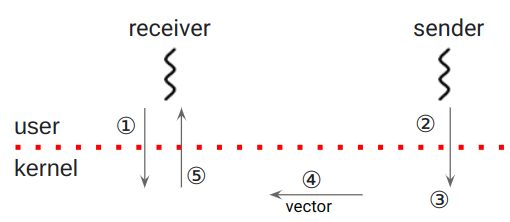
\includegraphics[width=\textwidth]{images/interruptSend.png}
  \caption{L'envois d'une interruption}
  \label{fig:sendInt}
\end{figure}

Lors du déclenchement du handler noyau certain registres actuelle sont sauvegardé comme le pointeur de pile \code{RSP}, le registre d'états \code{RFLAGS}, le registre \code{CS} et le registre de pointeur d'instruction \code{RIP}.
Cette sauvegarde ce fait en les empilant dans une nouvelle pile. Le vecteur de l'interruption est aussi empilé en temps que code erreur \emph{errorCode}.
Une fois que le handler noyau a fini de s'exécuter il doit faire l'instruction \code{iret} qui a pour effect de dépilé les registre sauvegardé et de les restorer.

Il est possible de masquer les interruptions grâce à deux instructions utilisable seulement par le noyau qui sont \code{clui} et \code{stui}.
Ces interruption modifie un flag (\emph{IF}) qui ce trouve dans le registre d'états de l'unité de calcul \code{RFLAGS} (aussi nommé \code{EFLAGS} sur les architecture 32bits).
La liste des instructions pour les IRQ ce trouve ici\ref{tab:interruptInstructions}.

Comme on la vue ce mécanisme fonctionne totalement dans le noyau du système.
Dans notre exemple il faut au minimum deux changement de contexte (context switch) pour le récepteur et l'émetteur et même peut être plus si le récepteur dois déclenché un handler coté utilisateur.

% Il fau noté que les registre 32 bit commance par un E et les 64 bit par un R (ex: EIP et RIP).
% RIP is Register Instructions Pointer, RFLAGS is Register with all core FLAGS (OF, CF, IF...), RSP is Register Stack Pointer, CS is Code Section, IF is Interrupt Flag store in EFLAGS

\subsubsection{Les uintr}
\label{sec:uintrDetails}

Le mécanisme d'interruption en espace utilisateur est utilise cinque nouvelle instructions qui sont listé dans le tableau suivant \ref{tab:interruptInstructions}.
Les deux premiers, \code{clui} et \code{stui}, permet le masquage des interruption, en effet comme pour les interruptions ordinaire qui on un flag \emph{IF} pour Interrupt Flag les uintr on un flag \emph{UIF} pour User Interrupt Flag.
l'instruction suivant \code{testui} permet à l'utilisateur de savoir si les interruption sont masquer ou non.
Cette instruction existe car l'utilisateur n'a pas accès directement au \emph{UIF} contrairement au interruption ordinaire ou le noyau a lui accès directement au \emph{IF}.
L'instruction suivant \code{uiret} fonctionne comme celle des interruption ordinaire (\code{iret}) mais pas avec les même registre et surtout elle est utilisable en espace utilisateur.
La dernier instruction permet d'envoyer une uintr grâce à un indice que nous allons voir dans cette section \ref{sec:exemple}.

\begin{figure}[H]
  \begin{tabular}{|l|l| }
    \hline
    \bf Interruption & \bf Interruption utilisateur\\
    \hline
    cli (\textbf{CL}ear \textbf{I}F) & clui (\textbf{CL}ear \textbf{UI}F)\\
    \hline
    sti (\textbf{S}e\textbf{T} \textbf{I}F) & stui (\textbf{S}e\textbf{T} \textbf{UI}F)\\
    \hline
    & testui (Read \textbf{UI}F)\\
    \hline
    iret (Interrupt RETurn) & uiret (User Interrupt RETurn)\\
    \hline
    \multirow{3}{0.5\textwidth}{APIC pins, APIC ICR, \code{INT n}, \code{INT3}, \code{INTO}, \code{BOUND} et \code{INT80 n}} & sendipi <uipi_index>\\
    &\\
    &\\
    &\\
    \hline
    % \multicolumn{2}{|c|}{...} \\
    % \hline
  \end{tabular}
  \caption{Instructions des interruption et interruption en espace utilisateur}
  \label{tab:interruptInstructions}
\end{figure}

Le mécanisme arrive aussi avec six nouveaux \emph{registres d'états}, des registres \emph{MSR} pour Model-specific registers.
Ces registres sont modifier par le noyau grâce à des appels système que l'utilisateur fait pour initialiser les uintr et utiliser par le CPU.
Ils sont décrit dans le tableau suivant\ref{tab:uintrStateRegisters} et nous expliciterons leur utilité par la suite.

\begin{figure}[H]
  \begin{tabular}{|l|l| }
    \hline
    \bf Nom du registre & \bf Description\\
    \hline
    IA32_UINTR_STACKADJUST & \multirow{2}{0.5\textwidth}{Utilisé par le récepteur pour définir l'adresse de la pile alternative}\\ % remplacé "définir" par "que l'unité de calcule connaisse"
    &\\
    \hline
    IA32_UINTR_HANDLER & \multirow{2}{0.5\textwidth}{Utilisé par le récepteur pour définir l'adresse du handler uintr}\\
    &\\
    \hline
    IA32_UINTR_MISC & \multirow{7}{0.5\textwidth}{Utilisé par l'émetteur pour définir la taille de la \emph{UITT} et
    par le récepteur pour que l'APIC connaisse le vecteur d'interruption ordinaire qu'il dois reconnaître pour déclencher le handler uintr
    et le dernier bit pour le flag de masquage \emph{UIF}}\\
    &\\
    &\\
    &\\
    &\\
    &\\
    &\\
    \hline
    IA32_UINTR_PD & \multirow{2}{0.5\textwidth}{Utilisé par le récepteur pour définir l'adresse du \emph{UPID}}\\
    &\\
    \hline
    IA32_UINTR_RR & \multirow{3}{0.5\textwidth}{Utilisé par l'APIC pour \textit{lister} les vecteurs uintr qu'il dois envoyer au récepteur\emph{UPID}}\\
    &\\
    &\\
    \hline
    IA32_UINTR_TT & \multirow{2}{0.5\textwidth}{Utilisé par l'émetteur pour définir l'adresse de la \emph{UITT}}\\
    &\\
    \hline
    % \multicolumn{2}{|c|}{...} \\
    % \hline
  \end{tabular}
  \caption{Liste des six registre d'états des uintr}
  \label{tab:uintrStateRegisters}
\end{figure}

% interrupt invoked (push oldRSP, RFLAGS, CS, RIP, errorCode (IRQ vector value ?))
% IRET (pop errorCode, RIP, CS, RFLAGS, oldRSP)
% uintr invoked (push oldRSP, RFLAGS, RIP, UIRRV)
% uiret (pop UIRRV, RIP, RFLAGS, oldRSP)

\subsubsection{Capacités présente et futur}

Le mécanisme a une interface pour l'utilisateur similaire aux signaux \ref{sec:signal}.
Nous allons donc voir les capacités des uintr par comparaison à celle des signaux.

Tous d'abord le fonction des uintr ce fait au niveau des threads que les signaux le fonctionnement ce fait au niveau du processus.
Il est possible d'avoir un fonctionnement qui ce rapproche d'un fonctionnement par threads avec plusieurs options.

Avec les uintr il est possible de définir une handler différant par threads d'un processus que pour les signaux il est possible de définir un seul handler pour tous les threads d'un processus.
Par-contre les signaux permet de définir un handler différant par signal se qui n'est pas possible avec les uintr, il faut le faire nous même en appelant la fonction qui correspond au vecteur reçus. %(le vecteur c'est une valeur qui est similaire au numéro de signal)

Il exit 64 signaux possible avec les 32 premiers qui on on signification, pour les uintr il existe aussi 64 vecteurs possible entre 0 et 63 qui n'ont aucune signification par défaut.

Pour les uintr le masquage ce fait via une instruction que pour les signaux il faut faire un appel système.

L'envois d'un signal ce fait par le noyau suite à une exceptions, une décision du noyau ou la demande d'un processus grâce à un appel système (\code{kill(signum)} ou \code{tgkill(signum)}).
Pour les uintr l'envoi peut ce faire depuis un autre processus ou depuis le noyau et dans le future pourra ce faire depuis un périphériques.

Avec les signaux le handler peut être déclenché que le processus cible soit endormi ou non pour les uintr c'est différant.
Il faut que le thread sois en espace utilisateur pour recevoir une interruption sinon l'interruption sera reçus quand le thread revient en espace utilisateur.
On a vue plutôt, dans les prérequis\ref{requirements}, qu'une fonctionnalité existe à la compilation du noyau pour autorisé l'interruption d'un thread bloqué.
Si la fonctionnalité est activé il est donc possible d'interrompre un thread qui n'est pas ordonnancer ou qui est entrain de faire un appel système interruptible et donc le passé en espace utilisateur pour qu'il puisse recevoir l'interruption. % tâche interruptible c'est plus précis mais il faut le mettre dans le context
Pour utilisé cette fonctionnalité l'utilisateur dois renseigné un flag au moment de définir le handler.
Il existe donc trois flags, le premier \code{UINTR_HANDLER_FLAG_WAITING_ANY} qui active la fonctionnalité et les deux autre qui s'ajoute au précédent et précise si c'est l'émetteur ou le récepteur qui vas prendre le surcoût du passage dans le noyau.
Les flags sont \code{UINTR_HANDLER_FLAG_WAITING_RECEIVER} et \code{UINTR_HANDLER_FLAG_WAITING_SENDER}.

Pour les signaux le déclenchement du handler est géré par le noyau qui vas sauvegarde de l'états du processus, définir une pile alternative si besoin, changer de context et appelé le handler utilisateur.
Pour les uintr le déclenchement du handler est fait par le CPU, il est donc très sommaire :
\begin{itemize}
  \item changer la pile si une pile alternative est disponible dans le registre \code{IA32_UINTR_STACKADJUST}
  \item empiler l'ancien pointeur de pile, le registre d'états de l'unité de calcul, le registre de pointeur d'instruction \code{RIP} et le vecteur uintr
  \item aller à l'adresse du handler utilisateur disponible dans le registre\\
  \code{IA32_UINTR_HANDLER}
\end{itemize}
C'est donc à l'utilisateur qu'appartient la responsabilité de la sauvegarde des registres généraux, des registres vectoriel (SIMD)... et des les restorer à la sortie du handler.
Le compilateur permet déjà de faire la sauvegarde des registres généraux avec le flag \code{general-regs-only} par-contre pour les registres vectoriel il faut les sauvegardé avant de les utilisé.
Il faut faire attention aux operations sur les chaîne de caractère de la \emph{libc} car \code{memcpy}, \code{memmove}, \code{memset} et \code{memcmp} utilise des registres vectoriel par défaut.
Le compilateur fournis le flag \code{-minline-all-stringops} qui permet d'inline\footnote{besoin d'expliqué l'inline?} ces opérations pour ne plus utiliser de registre vectoriel.

Une fois que le handler à fini sont execution il faut s'occuper du retour. Pour les signaux c'est le noyau qui s'en occupe et pour les uintr il faut que l'utilisateur utilise l'instruction \code{uiret}.
Donc l'unité de calcul vas dépilé le vecteur, les registers qui suivent pour les restorer ce qui vas permettre au code de continuer là où il en été.

Que ce sois dans un handler de signal ou dans un handler d'interruption utilisateur on a la même contrainte, on ne peu pas faire d'attente donc on peut seulement appeler le fonction et appel système dit \emph{async safe}.

\subsubsection{Exemple de fonctionnement}
\label{sec:exemple}

Nous allons maintenant voir un example d'initialisation des unitr montré sur la figure suivante \ref{fig:initUintr}.

\begin{enumerate}[label=\protect\circled{\arabic*}]
  \item Le récepteur enregistre au prés du noyau un handler d'interruption qu'il a défini.
  Le noyau vas enregistré ce handler dans le registre \code{IA32_UINTR_HANDLER} et vas initialiser une zone mémoire nommé \emph{UPID} pour User Posted Interrupt Descriptor.
  Ce \emph{UPID} permet au mécanisme des uintr de manipuler des informations propre à ce thread qui sont essentielle pour l'envoi d'uintr.
  Il est enregistré dans le registre \code{IA32_UINTR_PD}.
  \item Le récepteur donne au noyau un vecteur entre 0 et 63 qu'il veut recevoir, 8 dans la figure. Le noyau lui retourne un descripteur de fichier qui pointe vers une structure qui possède à la fois le vecteur et l'adresse du \emph{UPID}.
  \item Le récepteur envois ce descripteur de fichier aux émetteurs potentielle, un seul dans notre cas. Nous verrons comment partagé ce descripteur de fichier dans une section dédier\ref{sec:shareFD}.
  \item L'émetteur vas s'enregistrer au prés du noyau grâce au descripteur de fichier.
  Pour ce faire le noyau possède un tableau \emph{UITT} pour User Interrupt Target Table qui fait une taille de 256 entré par défaut.
  L'adresse de ce tableau dois être enregistré dans le registre \code{IA32_UINTR_TT} avec ça taille dans les 4 premier octets du registre \code{IA32_UINTR_MISC}, on peut donc faire varier la taille de ce tableau.
  Chaque entrées de ce tableau consiste en une zone mémoire nommé \emph{UITTE} pour User Interrupt Target Table Entry.
  Le noyau vas donc trouvé une entré libre dans le \emph{UITT} et renseigné l'\emph{UITTE} avec le vecteur et l'adresse du \emph{UPID} obtenu grâce au descripteur de fichier.
  Pour finir il retourne l'indice de l'entré à l'émetteur.
  \item L'utilisateur peut maintenant envoyer autant d'interruption totalement depuis l'espace utilisateur.
\end{enumerate}

\begin{figure}[H]
  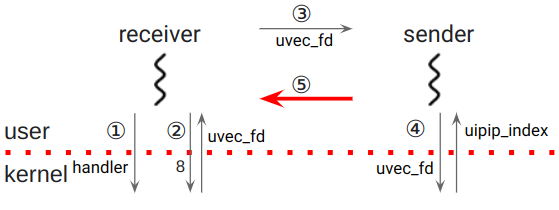
\includegraphics[width=\textwidth]{images/uintrInit.png}
  \caption{Phase d'initialisation des uintr}
  \label{fig:initUintr}
\end{figure}

\begin{figure}[H]
  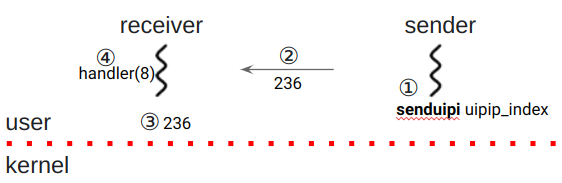
\includegraphics[width=\textwidth]{images/uintrSend.png}
  \caption{L'envois d'une uintr}
  \label{fig:sendUintr}
\end{figure}

\subsubsection{Partage du descripteur de fichier}
\label{sec:shareFD}

\begin{itemize}
  \item Pour mes testes "jouer" j'ai utiliser \verb|uintr_register_self()|
  \item pipe / socket / URL pour NewMadeleine (on en reparle en section XXX)
  \item inheritance / pidfd_getfd / sockets
  \item \verb|pidfd_getfd|
\end{itemize}

\subsection{Tests du mécanisme}

% sur un exemple minimal en communication inter-processus

\begin{itemize}
  \item entre process
  \item entre threads
  \item avec alt stack
  \item test d'écrasement des interruptions
  \item avec binding (plus pourquoi avec binding que comparaison avec et sans)
  \item avec turbo boost
\end{itemize}

TODO: on peut actuellement enregistré plusieurs fois la même FD donc avoir des UITTE en double...

\subsection{Correction du patch pour l'appel système uintr_alt_stack}

TODO

\subsection{Mesure de la latence (Feedback Mathieu)}

TODO: expliquer que le binding est important

\subsection{Performances}

TODO

\begin{itemize}
  \item Dans un premier temps j'ai pas bind les thread par pu donc j'avais de mauvais résultats.
  \item J'ai fait différents bind (on vois que c'est similaire sauf quand on passe entre 2 NUMA)
  \item si on monte la frequence c'est mieux (turbo boost)
  \item comparé au signaux...
\end{itemize}

je n'ai pas fait de test dans le cas ou le thread est endormi ou bloqué
